\question{Автоэлектронная эмиссия. Уравнение Фаулера-Нордгейма}

Эмиссию электронов из металла или полупроводника можно получить и без нагрева 
материала путем повышения напряженности электрического поля. В этом случае 
эмиссия происходит по иным физическим законам, в ее основе лежит 
квантово-механический эффект туннелирования электронов сквозь потенциальный 
барьер. Катод (эмиттер) остается холодным.

Рассмотрим, как изменяется поле на границе металл-вакуум (рис.\ref{img04.1}) 
при приложении большого по величине электрического поля. Примем, что 
потенциальная энергия внутри металла \( U(x) = 0 \), а вне металла 
\( W_B > 0 \). Это предположение соответствует гипотезе свободных электронов, 
когда внутри металла нет сил, действующих на электрон. Хотя с точки зрения 
квантово-механических представлений данное предположение не является строгим, 
его можно взять за основу.

Распределение по энергиям электронного газа в металле таково, что подавляющее 
большинство электронов имеет энергию \( E < W_B \). При температуре 
абсолютного нуля заполнены уровни от \( E = 0 \) до \( E = W_{F0} \) -- до 
уровня Ферми. Когда внешнего электрического поля нет (\( E_0 = 0 \)), то поток 
электронов, падающий изнутри металла на поверхность, полностью отражается от 
скачка потенциала \( W_B \).

Однако при наложении внешнего электрического поля, направленного к поверхности 
металла (\( E_0 \) -- величина напряженности электрического поля), к 
потенциальной энергии \( U(x) \) добавляется потенциальная энергия \( -eEx \) 
и полная энергия электрона будет равна:
\begin{equation}
	\begin{array}{cr}
		U_1(x) = U(x) - eE_0 x = W_B - eE_0 x & \text{при } x > 0 \\
		U_1(x) = 0 & \text{при } x < 0
	\end{array}
	\label{eq04.1.10}
\end{equation}
 
Изменение \( U(x) \) происходит лишь вне металла. Образуется потенциальный 
барьер, коэффициент прозрачности которого равен:
\begin{equation}
	S = \int\limits_{x_1}^{x_2} \sqrt{2m[qU(x)-W]}dx
	\label{eq04.1.11}
\end{equation}
где \( W \) -- энергия электронов внутри металла. Первая граничная точка 
\( х_1 = 0 \), так как для всякой энергии \( W < W_B \) горизонтальная прямая 
\( W \), изображающая движение по \( 0x \), пересекает кривую потенциальной 
энергии в точке \( x_1 = 0 \). Вторая точка получается при 
\( W = W_B - eE0x \) (рис.\ref{img04.1}). Отсюда

\begin{figure}[h]
    \center
    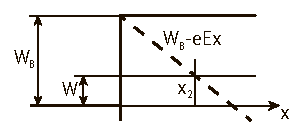
\includegraphics[width=.47\textwidth]{04_1}
    \caption{Упрощенная форма потенциального барьера для плоских электродов}
    \label{img04.1}
\end{figure}
 
Следовательно,
\[
	S = \int\limits_{0}^{\frac{W_B - W}{eE_0}} \sqrt{2m[W_B-eE_0 x - W]}dx = 
		\frac{2}{3}\sqrt{2m}\frac{(W_B-W)^{3/2}}{eE_0}
\]
и вероятность преодоления потенциального барьера равна:
\begin{equation}
	D(W) = D_0 \exp\left( -\frac{4\pi S}{h} \right) = 
		D_0 \exp\left[ -\frac{8\pi\sqrt{2m}(W_B-W)^{3/2}}{3ehE_0} \right]
	\label{eq04.1.13}
\end{equation}

Общее число электронов, эмитируемых вследствие туннельного эффекта, и, 
следовательно, плотность тока автоэлектронной эмиссии, получим, определив 
количество электронов, движущихся к поверхности металла с энергией, лежащей в 
диапазоне энергий от \( W \) до \( W + dW \). Для исключения теплового 
движения положим, что \( T = 0 \). Тогда, поскольку весь диапазон энергий 
лежит в интервале от \( 0 \) до \( W_{F0} \), можно производить интегрирование 
в интервале скоростей от \( 0 \) до \( v_F = \sqrt{2W_{F0}/m} \), поскольку 
самая простая функция распределения записывается в пространстве скоростей.

При \( T = 0 \) К электроны в пространстве скоростей располагаются с 
равномерной плотностью, образуя шар радиуса \( v_F \). Поскольку эмиссию 
обеспечивают лишь частицы, имеющие составляющие скорости, нормальные к 
поверхности металла (в нашем случае вдоль направления \(ОХ\)), число 
электронов, ударяющихся о границу металла и имеющих скорости от \( v_x \) до 
\( v_x + dv_x \), получим, определив количество электронов, приходящихся на 
этот интервал скоростей. Для оценки этой величины обратимся к 
рис.\ref{img04.2}. Объем шарового слоя, соответствующий заштрихованной зоне 
(интервал скоростей от \( v_x \) до \( v_x + dv_x\)) равен 
\( \pi(v^2_F - v^2_x)dv_x \). Поскольку объем элементарной ячейки, 
приходящейся на один электрон, равен \( h^3 / 2m^3 \), концентрация электронов 
равна \( 2\pi(m/h)^3 (v^2_F - v^2_x)dv_x \), а число электронов, ударяющихся о 
единичную поверхность за единицу времени, определяется так:
\begin{equation}
	dN = 2\pi\left( \frac{m}{h} \right)^3 v_x \left( v^2_F - v^2_x \right)dv_x
	\label{eq04.1.14}
\end{equation}

\begin{figure}[h]
    \center
    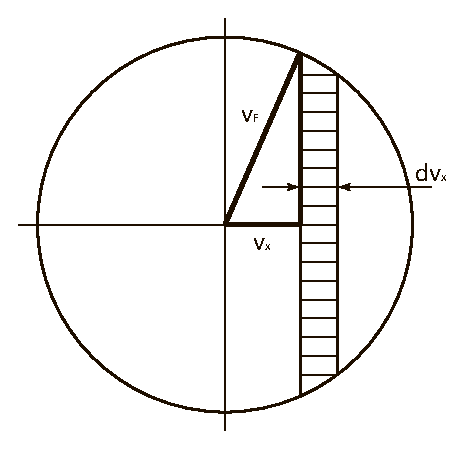
\includegraphics[width=.47\textwidth]{04_2}
    \caption{Схема расчёта числа электронов, ударяющихся о граничную 
    	поверхность металла при \( T = 0 \) К}
    \label{img04.2}
\end{figure}
Следовательно, общее число электронов, вылетающих за пределы металла, 
определяется с учетом вероятности прохождения ими потенциального барьера:
\begin{equation}
	N = 2\pi\left( \frac{m}{h} \right)^3 \int\limits_{0}^{v_F} 
		D_0 v_x \left( v^2_F - v^2_x \right) 
		\exp\left[ -8\pi\frac{\sqrt{2m}}{3eh} 
		\left( W_D - \frac{mv^2_x}{2} \right)^{3/2} \right] dv_x
	\label{eq04.1.15}
\end{equation}

Здесь введено, что \( W = mv^2_x / 2 \). Множитель \( D_0 \) является 
амплитудой коэффициента прозрачности барьера -- отношения потока прошедших 
частиц к потоку частиц, падающих на барьер. Он зависит от соотношения величин 
энергий частиц и высоты барьера:
\begin{equation}
	D_0 = \frac{16W(W_B-W)}{W^2_B}
	\label{eq04.1.16}
\end{equation}
и мало отличается от единицы.

В результате интегрирования уравнения (\ref{eq04.1.15}) получается формула 
Фаулера–Нордгейма для плотности тока автоэлектронной эмиссии:
\begin{equation}
	J_E = \frac{6.210^{-6}}{W_B}\left( \frac{W_{F0}}{W_A} \right)^{1/2}
		E^2_0 \exp\left[ -6.810^9 \frac{W_A^{3/2}}{E_0} \right]
	\label{eq04.1.17}
\end{equation}
в которой для удобства подставлены все физические константы: \( W_A \) -- 
работа выхода из металла, \( E_0 \) измеряется в В/м, \( W_A \) и \( W_B \) -- 
в эВ, а плотность тока получается в А/м.

Несмотря на достаточно грубые приближения, введенные при выводе формулы 
(\ref{eq04.1.17}), в ряде случаев для различных материалов получаются расчеты, 
достаточно хорошо совпадающие с экспериментальными результатами.

Величина плотности тока автоэлектронной эмиссии сильно зависит от 
напряженности электрического поля. Так, например, для вольфрама при 
напряженности внешнего электрического поля \( E_0 = 2\cdot10^9 \) В/м 
плотность тока составляет \( 5 \) А/м, а уже при \( E_0 = 4\cdot10^9 \) В/м 
она равна \( 10^8 \) А/м.

В современной электронике автоэлектронные катоды используются достаточно 
широко.
